\chapter{swash\_solution}

%NSLW Equations:Analytical Solutions
%HR Wallingford Internal Workshop
%Dr.D.M.Kelly
%November 2010
%Chapter2: 2.1 Ritter Dam-break Solution

\section{Description}

The configuration is a 8~m long and 0.5~m wide rectangle.

\subsection{Geometry and mesh}

The mesh is made of 7,317 elements and 3,908 nodes
(see Figure~\ref{fig:swash:mesh}).

\begin{figure}[H]
\centering
\includegraphicsmaybe{[width=.9\textwidth]}{../img/Mesh.png}
\caption{Mesh of the study.}
\label{fig:swash:mesh}
\end{figure}

Figure~\ref{fig:swash:bathy} displays the bathymetry.

\begin{figure}[H]
\centering
\includegraphicsmaybe{[width=.9\textwidth]}{../img/Bathy.png}
\caption{Bathymetry of the study.}
\label{fig:swash:bathy}
\end{figure}

\subsection{Boundaries}

Figure~\ref{fig:swash:boundaries} shows the boundaries of the study.

\begin{figure}[H]
\centering
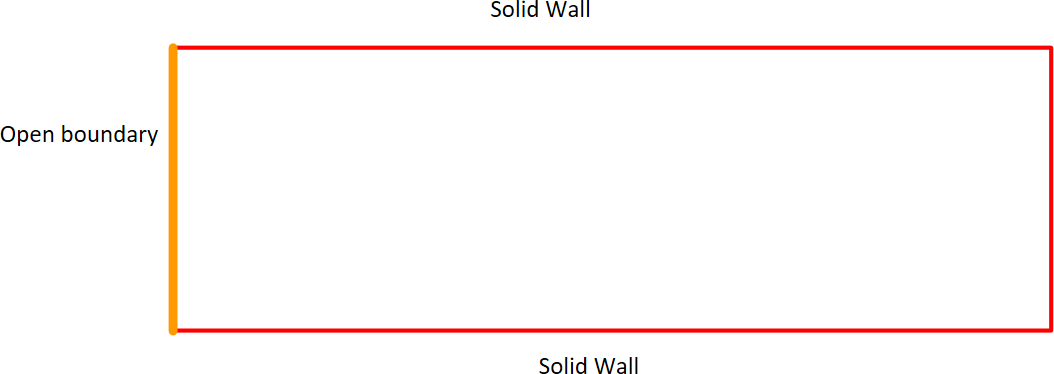
\includegraphics[width=.9\textwidth]{img/boundaries.png}
\caption{Boundaries of the study.}
\label{fig:swash:boundaries}
\end{figure}

Wave generated for $x$ > 6~m:
\begin{equation}
H(x) = \frac{x}{20}+\frac{0.05}{\cos(\arctan(0.05))}
\end{equation}

Bottom: No bottom friction

\subsection{Physical parameters}

Turbulence: Constant viscosity equal to zero

\subsection{Numerical parameters}

%Saint Venant VF Equations
\begin{itemize}
\item Type of element: P1 triangle for $h$ and for velocity,
\item Type of advection: Implicit N scheme on non conservative equation + SUPG decentring on velocities PSI distributive scheme, mass-conservative + modified SUPG on depth,
\item Solver: GMRES,
\item Accuracy: 10$^{-4}$,
\item Finite volume scheme: Kinetic order 2,
\item Implicitation for depth: 1,
\item Implicitation for velocity: 0.6.
\end{itemize}

Time data:
\begin{itemize}
\item Desired Courant number = 0.8,
\item Simulation duration: 12~s.
\end{itemize}

\section{Results}

Figure~\ref{fig:swash:vel} shows the velocity vectors.

\begin{figure}[H]
\centering
\includegraphicsmaybe{[width=.9\textwidth]}{../img/FreeSurface.png}
%The fixed figure is not exactly the same as the automatically generated one
%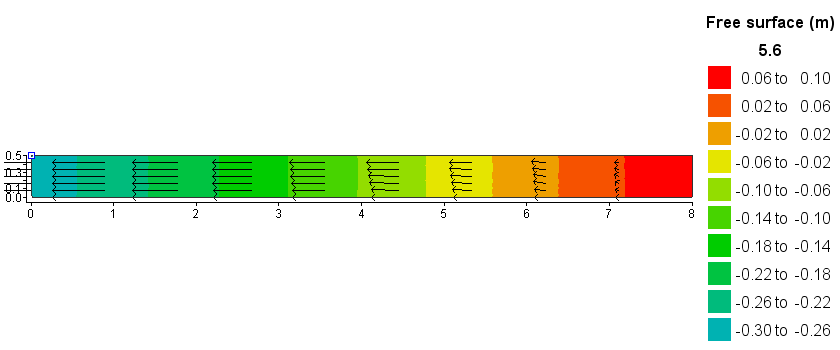
\includegraphics[width=\textwidth]{img/vel.png}
\caption{Velocity vectors and free surface.}
\label{fig:swash:vel}
\end{figure}

We then compare the model and the analytical solution free surface.

Figure~\ref{fig:swash:res} shows the comparison for the free surface.

\begin{figure}[H]
\centering
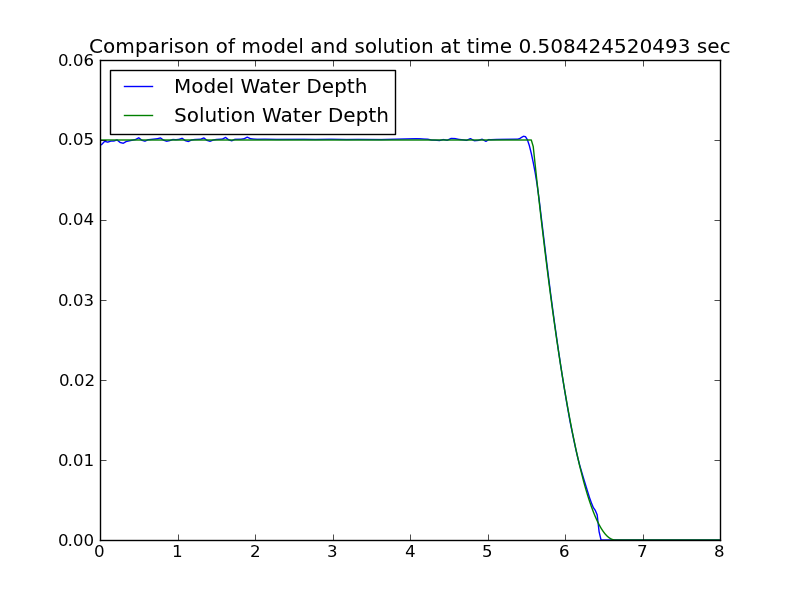
\includegraphics[width=.5\textwidth]{img/res_t0_5.png}
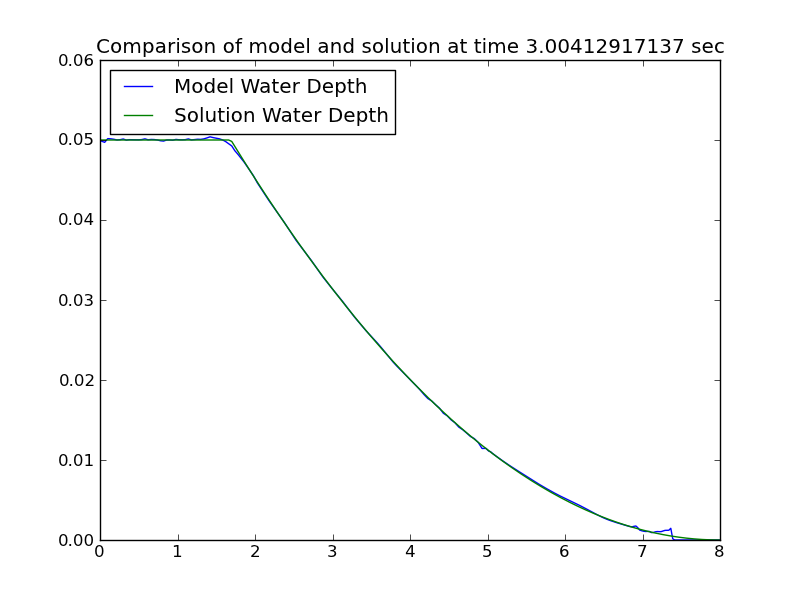
\includegraphics[width=.5\textwidth]{img/res_t3_0.png}
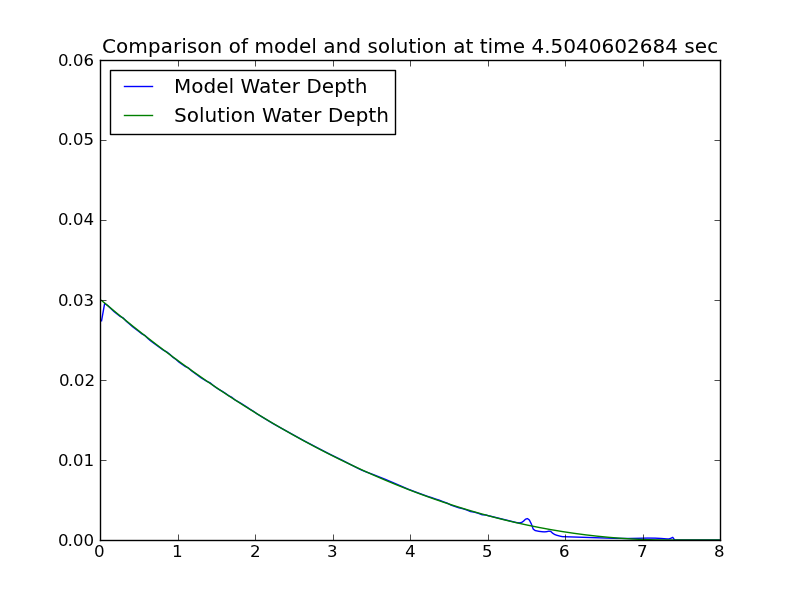
\includegraphics[width=.5\textwidth]{img/res_t4_5.png}
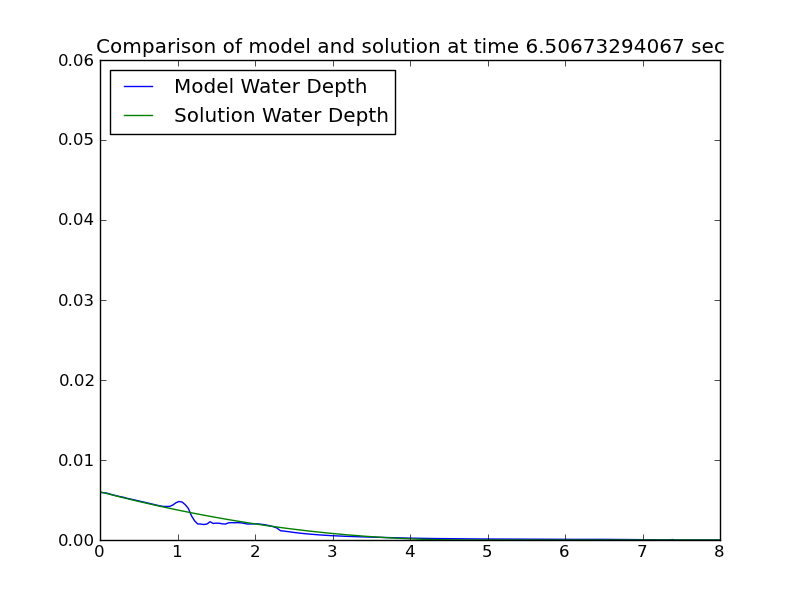
\includegraphics[width=.5\textwidth]{img/res_t6_5.png}
\caption{Comparaison of the results.}
\label{fig:swash:res}
\end{figure}

Figure~\ref{fig:swash:res_vel} shows the comparison for the velocity.

\begin{figure}[H]
\centering
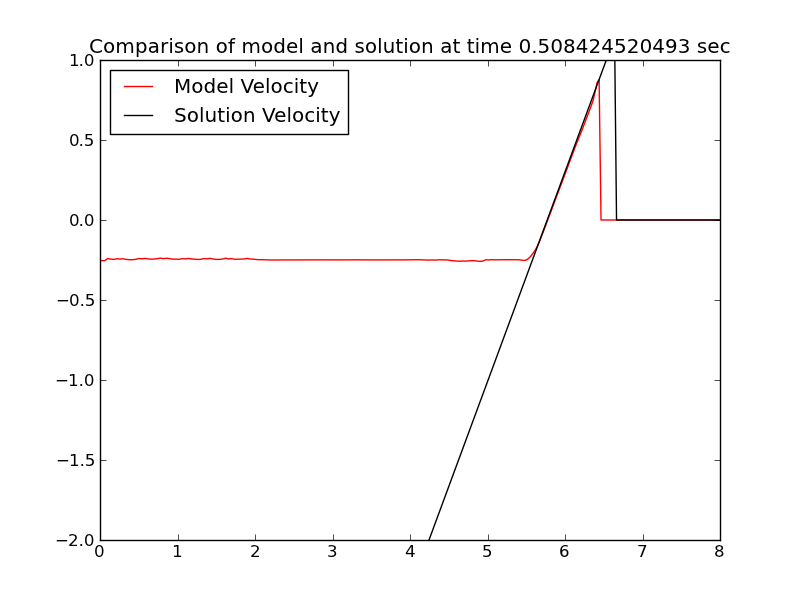
\includegraphics[width=.5\textwidth]{img/res_vel_t0_5.png}
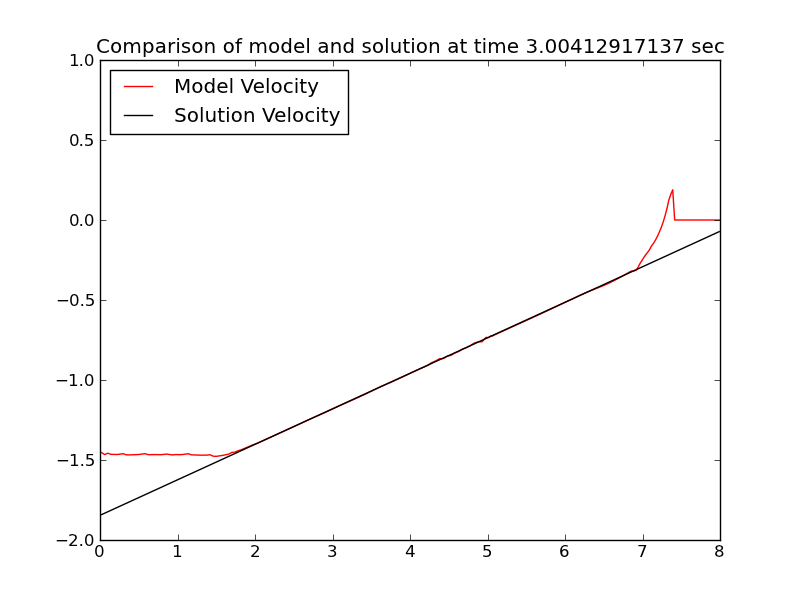
\includegraphics[width=.5\textwidth]{img/res_vel_t3_0.png}
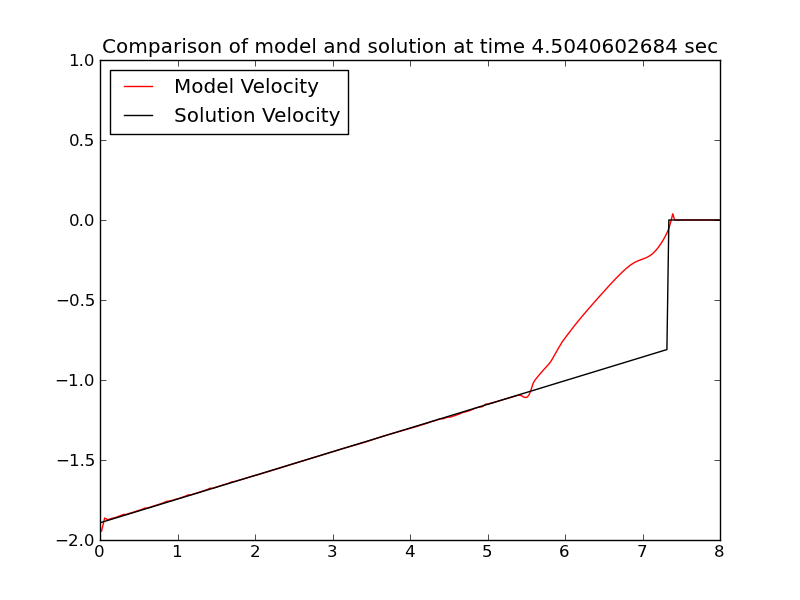
\includegraphics[width=.5\textwidth]{img/res_vel_t4_5.png}
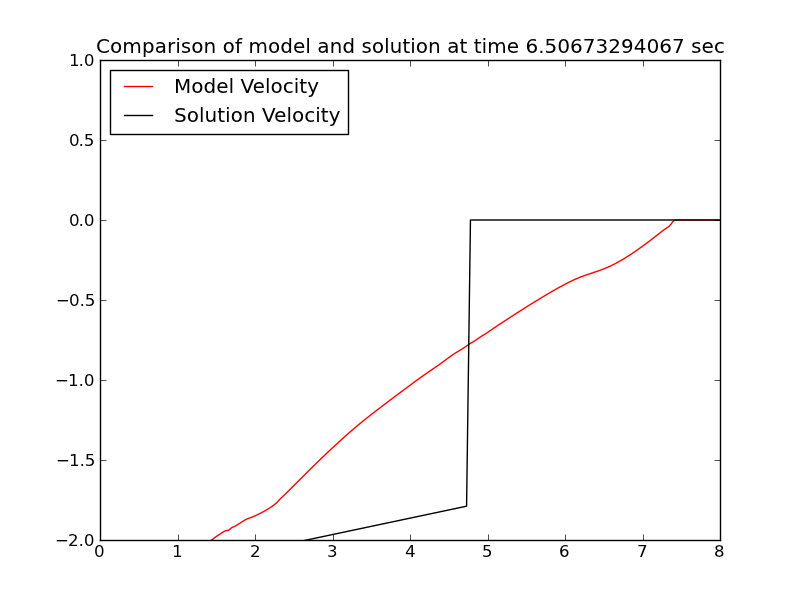
\includegraphics[width=.5\textwidth]{img/res_vel_t6_5.png}
\caption{Comparaison of the results for the velocity.}
\label{fig:swash:res_vel}
\end{figure}
